\documentclass[border=12pt]{standalone}
\usepackage{tikz}
\usetikzlibrary{shapes.geometric, arrows.meta, positioning, calc, fit, backgrounds}
\usepackage{fontspec}
\setmainfont{DejaVu Sans}

\begin{document}
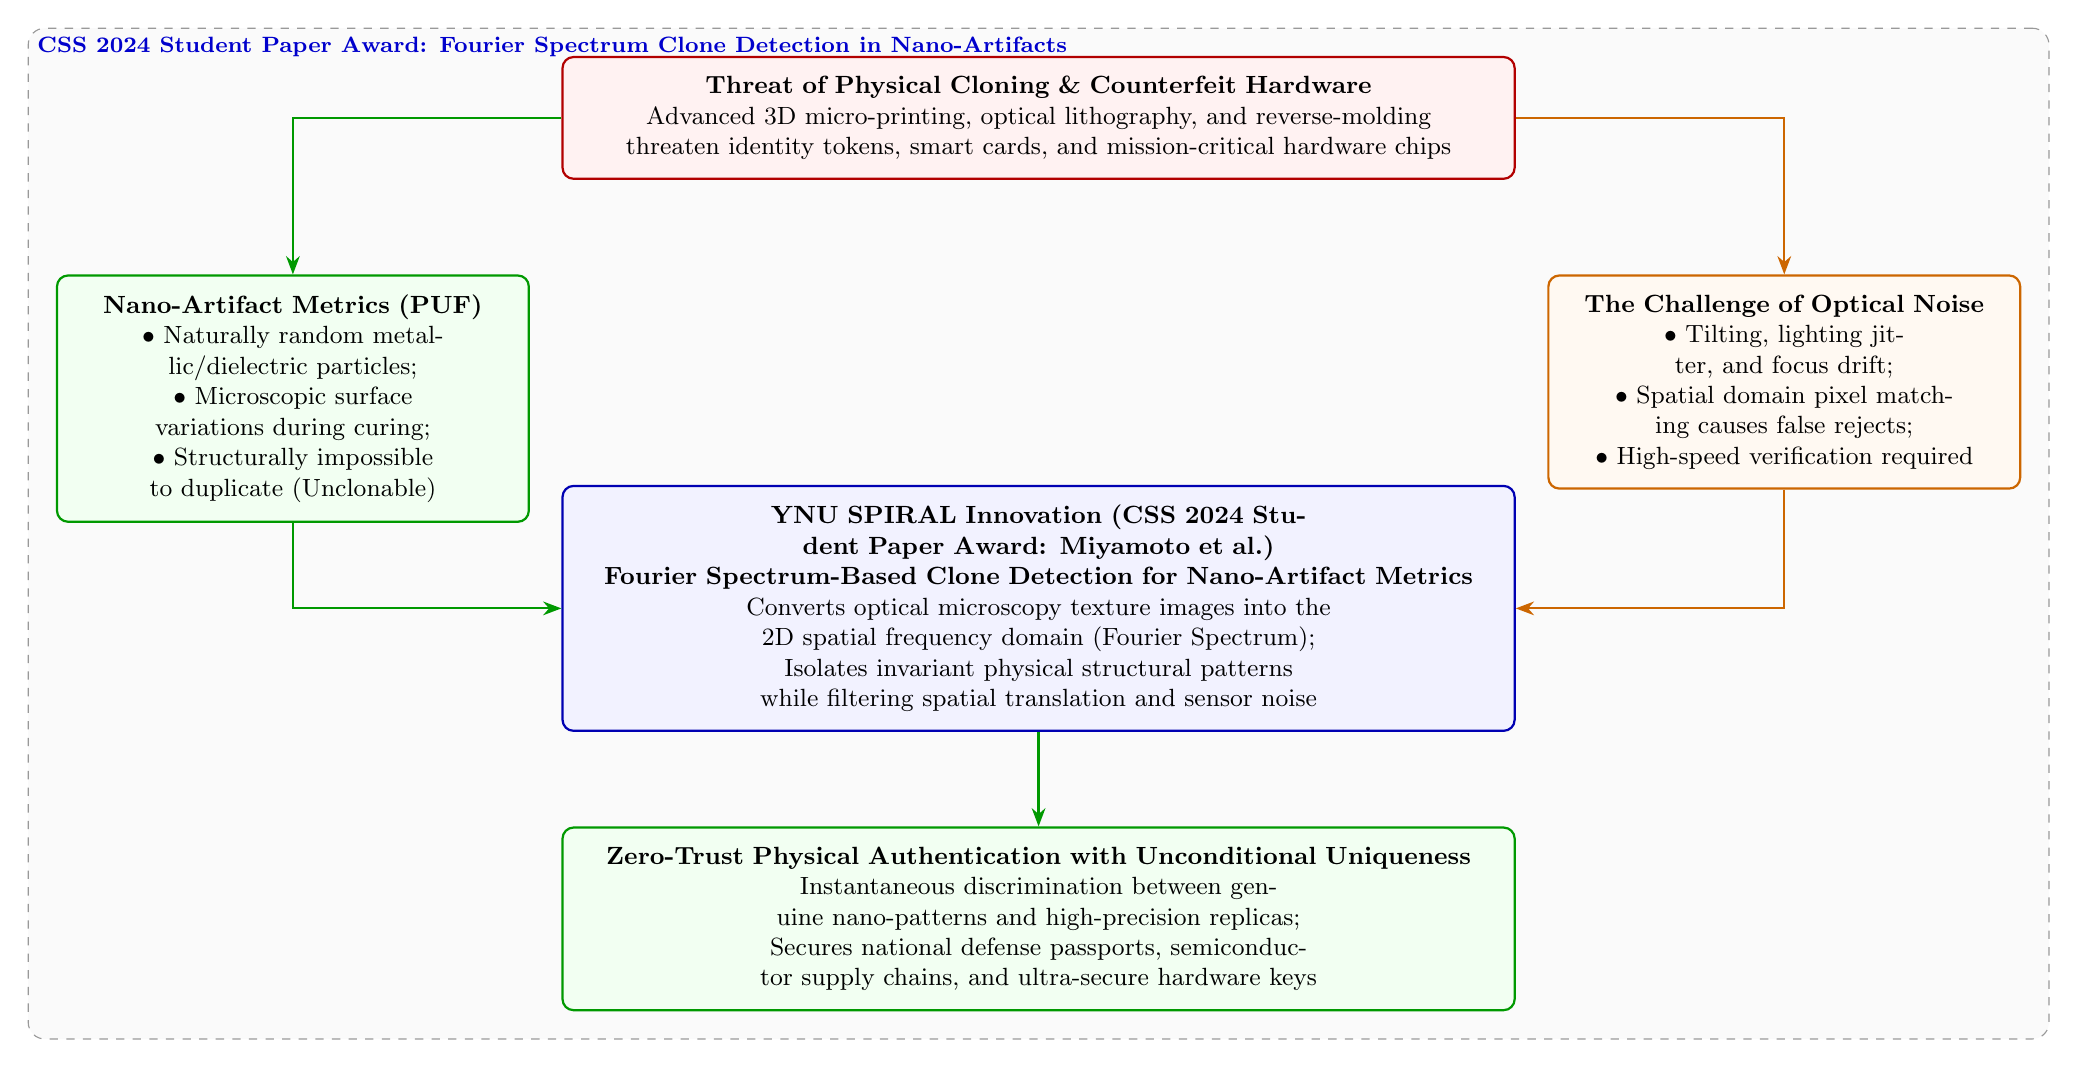
\begin{tikzpicture}[
    font=\small,
    >=Stealth,
    node distance=1.2cm,
    block/.style={rectangle, draw=blue!70!black, fill=blue!5, rounded corners=4pt, thick, align=center, inner sep=7pt},
    alertblock/.style={rectangle, draw=red!70!black, fill=red!5, rounded corners=4pt, thick, align=center, inner sep=7pt},
    greenblock/.style={rectangle, draw=green!60!black, fill=green!5, rounded corners=4pt, thick, align=center, inner sep=7pt},
    amberblock/.style={rectangle, draw=orange!80!black, fill=orange!5, rounded corners=4pt, thick, align=center, inner sep=7pt},
    groupbox/.style={draw=black!40, dashed, rounded corners=6pt, fill=black!2, inner sep=10pt}
]

    % Top: The Anti-Counterfeiting & Clone Threat
    \node[alertblock, text width=11.6cm] (counterfeit) {\textbf{Threat of Physical Cloning \& Counterfeit Hardware}\\Advanced 3D micro-printing, optical lithography, and reverse-molding\\threaten identity tokens, smart cards, and mission-critical hardware chips};

    % Left: Nano-Artifact Randomness
    \node[greenblock, below left=1.2cm and 0.4cm of counterfeit, text width=5.5cm] (nano) {\textbf{Nano-Artifact Metrics (PUF)}\\$\bullet$ Naturally random metallic/dielectric particles;\\$\bullet$ Microscopic surface variations during curing;\\$\bullet$ Structurally impossible to duplicate (Unclonable)};

    % Right: Challenge of Optical Reading Noise
    \node[amberblock, below right=1.2cm and 0.4cm of counterfeit, text width=5.5cm] (noise) {\textbf{The Challenge of Optical Noise}\\$\bullet$ Tilting, lighting jitter, and focus drift;\\$\bullet$ Spatial domain pixel matching causes false rejects;\\$\bullet$ High-speed verification required};

    \draw[->, thick, green!60!black] (counterfeit) -| (nano);
    \draw[->, thick, orange!80!black] (counterfeit) -| (noise);

    % Middle: YNU Innovation (CSS 2024 Student Paper Award: Miyamoto, Yoshida, Yoshioka, Matsumoto)
    \node[block, below=1.2cm of $(nano)!0.5!(noise)$, text width=11.6cm] (breakthrough) {\textbf{YNU SPIRAL Innovation (CSS 2024 Student Paper Award: Miyamoto et al.)}\\\textbf{Fourier Spectrum-Based Clone Detection for Nano-Artifact Metrics}\\Converts optical microscopy texture images into the 2D spatial frequency domain (Fourier Spectrum);\\Isolates invariant physical structural patterns while filtering spatial translation and sensor noise};

    \draw[->, thick, green!60!black] (nano) |- (breakthrough);
    \draw[->, thick, orange!80!black] (noise) |- (breakthrough);

    % Bottom: Impact
    \node[greenblock, below=1.2cm of breakthrough, text width=11.6cm] (impact) {\textbf{Zero-Trust Physical Authentication with Unconditional Uniqueness}\\Instantaneous discrimination between genuine nano-patterns and high-precision replicas;\\Secures national defense passports, semiconductor supply chains, and ultra-secure hardware keys};

    \draw[->, thick, green!60!black] (breakthrough) -- (impact);

    \begin{scope}[on background layer]
        \node[groupbox, fit=(counterfeit) (nano) (noise) (breakthrough) (impact), label={[anchor=north west, font=\footnotesize\bfseries, blue!80!black]north west:CSS 2024 Student Paper Award: Fourier Spectrum Clone Detection in Nano-Artifacts}] {};
    \end{scope}

\end{tikzpicture}
\end{document}
